
\section{Requirements Specification}
These requirements were decided on during the early stages of the project. The requirements have been split into several 
sections depending on their necessity

\subsection{Use Cases}
The core use cases for the system are:
\begin{itemize}
 \item Administration
 \subitem Login
 \subitem Logout
 \subitem View Status
 \subitem View Queries Frequency
 \subitem Change the way system updates academics
 \subitem Generate a custom look for university
 \subitem View publications details and visits statistics
 
 \item Common utility activities
 \subitem Search for experts with respect to a query
 \subitem View Academic Profile
 \subitem View relevant publications with respect to a query
 \subitem View relevant funded projects with respect to a query
\end{itemize}

\subsubsection{Actors}

\begin{figure}
\centering
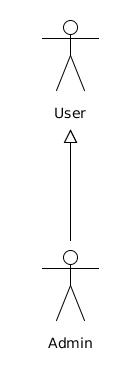
\includegraphics[scale=0.4]{./figures/actors.jpg}
\caption{Actors}
\end{figure}

\textbf{Figure 1} illustrates the relationships between actor roles in the system. A short summary of the actors is given below:

\textbf{User} represents an actor in the system who is able to search for experts with respect to a query. The search can be done via SICSA look
or university template look.

\textbf{Admin} inherits from user and is able to modify look and feel, update academics and view queries infromation.

\begin{figure}
\centering
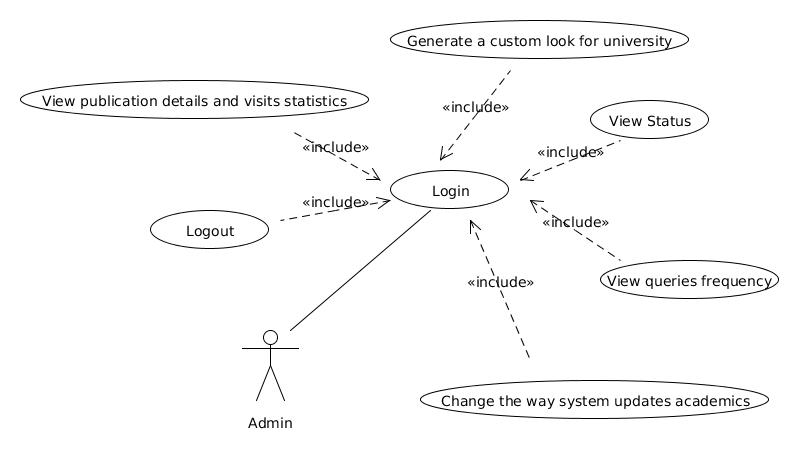
\includegraphics[scale=0.4]{./figures/use_case.jpg}
\caption{Administration Use Case Diagram}
\end{figure}

\textbf{Figure 2} illustrates the administration use case diagram of the system.

\subsection{Function Requirements}

\subsubsection{Administration}

%==============================================================================
% Logout

\begin{tabular}{|l|p{8.5cm}|}
\hline \textbf{Use Case} & Logout \\
\hline \textbf{Description} & The logout use case changes a user's status to logged out. Logout is invoked by the user \\
\hline \textbf{Rationale} & The logout use case allows a user to leave to system to prevent unauthorised use from an unattended terminal \\
\hline \textbf{Priority} & Must Have \\ 
\hline \textbf{Actors} & 
\begin{itemize}
 \item Admin
\end{itemize} \\
\hline \textbf{Includes} & Login \\
\hline \textbf{Conditions} & 
\begin{itemize}
 \item \textbf{post} The user is logged in
\end{itemize} \\ \hline
\end{tabular}

%==============================================================================
% Login

\begin{tabular}{|l|p{8.5cm}|}
\hline \textbf{Use Case} & Login \\
\hline \textbf{Description} & \raisebox{-\totalheight}{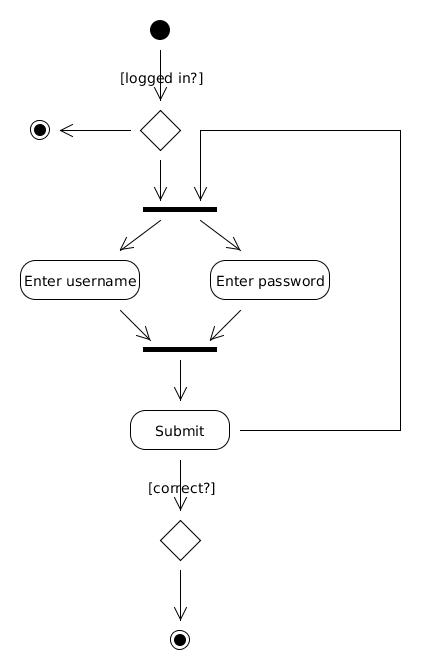
\includegraphics[scale=0.5]{./figures/login.jpg}} \\
\hline \textbf{Rationale} & The login use case allows administrator to access to the system. The usename and password are provided by SICSA staff \\
\hline \textbf{Priority} & Must Have \\ 
\hline \textbf{Actors} & 
\begin{itemize}
 \item Admin
\end{itemize} \\
\hline \textbf{Conditions} & \textbf{post} The user is logged in if correct credentials are provided \\  \hline
\end{tabular}

\vspace{10 mm}

%==============================================================================
% View Status

\begin{tabular}{|l|p{8.5cm}|}
\hline \textbf{Use Case} & View Status \\
\hline \textbf{Description} & A user's status (institution, email) is displayed \\
\hline \textbf{Rationale} & User needs to be able to view their status in the system \\
\hline \textbf{Priority} & Should Have \\ 
\hline \textbf{Actors} & 
\begin{itemize}
 \item Admin
\end{itemize} \\
\hline \textbf{Includes} & Login \\
\hline \textbf{Conditions} & 
\begin{itemize}
 \item \textbf{pre} The user is logged in
\end{itemize} \\ \hline
\end{tabular}

%==============================================================================
% View queries frequency

\begin{tabular}{|l|p{8.5cm}|}
\hline \textbf{Use Case} & View Queries Frequency \\
\hline \textbf{Description} & The submitted queries Frequency associated to user's institution is displayed \\
\hline \textbf{Rationale} & User needs to be able to view queries frequency in order to determine the popularity of particular areas \\
\hline \textbf{Priority} & Should Have \\ 
\hline \textbf{Actors} & 
\begin{itemize}
 \item Admin
\end{itemize} \\
\hline \textbf{Includes} & Login \\
\hline \textbf{Conditions} & 
\begin{itemize}
 \item \textbf{pre} The user is logged in
\end{itemize} \\ \hline
\end{tabular}

%==============================================================================
% Change the way system updates academics

\begin{tabular}{|l|p{8.5cm}|}
\hline \textbf{Use Case} & Change the way system updates academics \\
 \hline \textbf{Description} & Initially, the system scrapes the academics from user's webpage. Some users may prefer XML feeds from each university.
 There are currently 2 options: 
 \begin{itemize}
  \item an XML feed hosted on user's website and accessed directly by the system
  \item manual uploading of XML file to the system
 \end{itemize} \\
\hline \textbf{Rationale} & Allows user to upload academics in different ways \\
\hline \textbf{Priority} & Should Have \\ 
\hline \textbf{Actors} & 
\begin{itemize}
 \item Admin
\end{itemize} \\
\hline \textbf{Includes} & Login \\
\hline \textbf{Conditions} & 
\begin{itemize}
 \item \textbf{pre} The user is logged in
 \item \textbf{post} Change updated
\end{itemize} \\ \hline
\end{tabular}

%==============================================================================
% Generate custom look for university

\begin{tabular}{|l|p{8.5cm}|}
\hline \textbf{Use Case} & Generate a custom look for university \\
 \hline \textbf{Description} & User modifies look and feel of their university. This look and feel is displayed to other users visiting SICSA using 
 specific university look and feel \\
\hline \textbf{Rationale} & Allows user to modify template of their university \\
\hline \textbf{Priority} & Could Have \\ 
\hline \textbf{Actors} & 
\begin{itemize}
 \item Admin
\end{itemize} \\
\hline \textbf{Includes} & Login \\
\hline \textbf{Conditions} & 
\begin{itemize}
 \item \textbf{pre} The user is logged in
 \item \textbf{post} look and feel updated
\end{itemize} \\ \hline
\end{tabular}

%==============================================================================
% View publication details and visit statistics

\begin{tabular}{|l|p{8.5cm}|}
\hline \textbf{Use Case} & View publication details and visit statistics \\
 \hline \textbf{Description} & User is able to view all academics, number of visits and publications in their university \\
\hline \textbf{Rationale} & Allows user to view publication details and visit statistics \\
\hline \textbf{Priority} & Should Have \\ 
\hline \textbf{Actors} & 
\begin{itemize}
 \item Admin
\end{itemize} \\
\hline \textbf{Includes} & Login \\
\hline \textbf{Conditions} & 
\begin{itemize}
 \item \textbf{pre} The user is logged in
\end{itemize} \\ \hline
\end{tabular}


\subsubsection{Common Utility Activities}

\begin{figure}
\centering
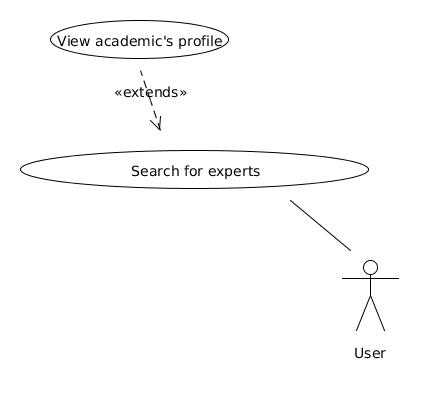
\includegraphics[scale=0.4]{./figures/common_utility_activities.jpg}
\caption{Common Utility Activities Use Case Diagram}
\end{figure}

\textbf{Figure 3} illustrates the common utility activities use case diagram of the system.

%==============================================================================
% Search for experts

\begin{tabular}{|l|p{8.5cm}|}
\hline \textbf{Use Case} & Search for Experts \\
\hline \textbf{Description} & \raisebox{-\totalheight}{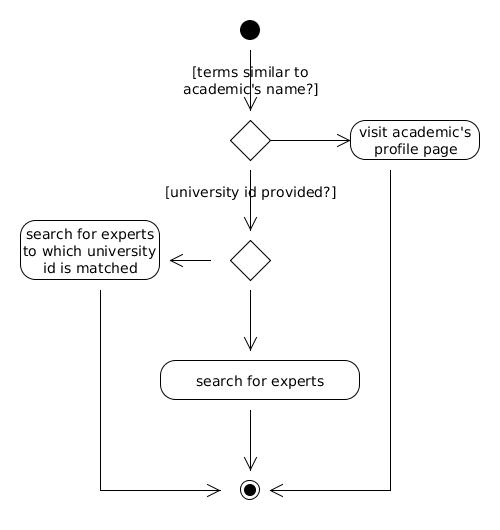
\includegraphics[scale=0.5]{./figures/search_for_experts.jpg}} 
User is able to search for experts. By default, all experts retrieved are ones whose university is registered to SICSA\\
\hline \textbf{Rationale} & Allows user to search for experts \\
\hline \textbf{Priority} & Must Have \\ 
\hline \textbf{Actors} & 
\begin{itemize}
 \item User
\end{itemize} \\ \hline
\end{tabular}

%==============================================================================
% View Academic's Profile

\begin{tabular}{|l|p{8.5cm}|}
\hline \textbf{Use Case} & View Academic's Profile \\
\hline \textbf{Description} & 

\raisebox{-\totalheight}{\centerline{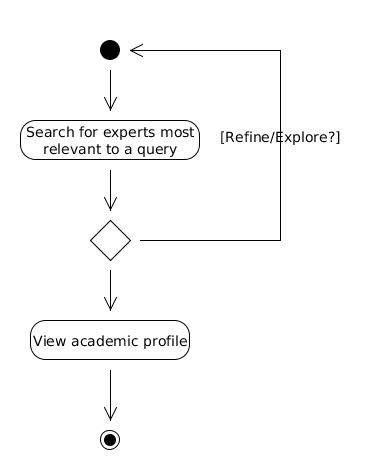
\includegraphics[scale=0.5]{./figures/view_academic_profile.jpg}}} 
The academic's profile's page includes
\begin{itemize}
 \item A list of publications most relevant to a query
 \item A list of funded projects most relevant to a query
 \item All publications of the academic
 \item All funded projects of the academic
 \item Most collaborated co-authors
 \item Most popular terms
 \item project's details (funding, funder, dates, academics)
\end{itemize} \\
\hline \textbf{Rationale} & Allows user to view academic's profile \\
\hline \textbf{Priority} & Must Have \\ 
\hline \textbf{Actors} & 
\begin{itemize}
 \item User
\end{itemize} \\
\hline \textbf{Extensions} & 
\begin{itemize}
 \item Search for experts
\end{itemize} \\ \hline
\end{tabular}

\subsection{Non-functional Requirements}
There are two sections of non-functional requirements which are Must Haves and Should Haves.

\subsubsection{Must Have}

\begin{tabular}{|l|p{8.5cm}|}
\hline \textbf{Effectiveness} & 
\begin{itemize}
 \item Help user find relevant experts by using publications and funded projects as expertise evidence
 \item Learn those expertise evidences using Learning to Rank Algorithm for Information Retrieval
\end{itemize} \\
\hline \textbf{Availability} & 
\begin{itemize}
 \item Functional 24 hours a day
\end{itemize} \\
\hline \textbf{Security} & 
\begin{itemize}
 \item Username and Password required for administrators
 \item Inactivity timeouts - 30 minutes
\end{itemize} \\
\hline \textbf{Performance} & 
\begin{itemize}
 \item Take less than a second to search for experts
 \item Take less than 3 seconds to visit academic's profile page
\end{itemize} \\ 
\hline \textbf{Documentation} & 
\begin{itemize}
 \item Administrator manual provided
\end{itemize} \\ 
\hline \textbf{Integrity} & 
\begin{itemize}
 \item Download data from DBLP database, Research to Gateway (GtR) and Grant on the Web (GoW) Spreadsheet.
 \item File System saved
\end{itemize} \\ 
\hline
\end{tabular}

\subsubsection{Should Have}
\begin{tabular}{|l|p{8.5cm}|}
\hline \textbf{Usability} &
\begin{itemize}
 \item Show evidence of the relevant experts with respect to a query
 \item Emphasise simplicity
 \item Fully functional for the purpose of the final demonstration
\end{itemize} \\
\hline \textbf{Recovery} & 
\begin{itemize}
 \item Update data regularly
\end{itemize}  \\ \hline
\end{tabular}



